% 建议使用 XeLaTeX 或 LuaLaTeX 编译(中文与公式支持更佳)
\documentclass[UTF8,zihao=-4]{ctexart}

\usepackage[a4paper,margin=2.5cm]{geometry}
\usepackage{amsmath, amssymb, amsthm}
\usepackage{bm}
\usepackage{hyperref}
\usepackage{graphicx}
\usepackage{caption}
\usepackage{listings}
\usepackage{xcolor}
\usepackage{float}
\usepackage{placeins}
\graphicspath{{figures/}}

\lstdefinestyle{code}{
  basicstyle=\ttfamily\small,
  numbers=left,
  numberstyle=\tiny,
  numbersep=8pt,
  keywordstyle=\color{blue},
  commentstyle=\color{teal!70!black},
  stringstyle=\color{orange!70!black},
  showstringspaces=false,
  breaklines=true,
  frame=single,
  framerule=0.3pt,
  rulecolor=\color{black!15}
}
\lstset{style=code}

\title{t-SNE:原理、公式、应用与实战}
\author{}
\date{\today}

\begin{document}
\maketitle

\section{引言}
t-分布随机邻域嵌入(t-Distributed Stochastic Neighbor Embedding, t-SNE)是一种非线性降维方法,用于将高维数据可视化到二维或三维。它通过将样本间距离转化为概率,并最小化原空间与嵌入空间邻域概率分布的 KL 散度,从而获得直观的簇结构。

\section{原理与公式}
\subsection{高维相似度}
对高维样本 \(\mathbf{x}_i\),t-SNE 定义条件概率衡量相邻关系:
\begin{equation}
p_{j|i} = \frac{\exp\left(-\lVert \mathbf{x}_i - \mathbf{x}_j \rVert_2^2 / 2\sigma_i^2\right)}{\sum_{k \neq i} \exp\left(-\lVert \mathbf{x}_i - \mathbf{x}_k \rVert_2^2 / 2\sigma_i^2\right)},
\end{equation}
其中 \(\sigma_i\) 通过二分搜索确定,使该分布的困惑度(perplexity)等于用户设定值。

\subsection{低维嵌入}
在嵌入空间中,t-SNE 采用自由度为 1 的学生 t 分布:
\begin{equation}
q_{ij} = \frac{\left(1 + \lVert \mathbf{y}_i - \mathbf{y}_j \rVert_2^2\right)^{-1}}{\sum_{k \neq l} \left(1 + \lVert \mathbf{y}_k - \mathbf{y}_l \rVert_2^2\right)^{-1}}.
\end{equation}
优化目标为对称化的 KL 散度:
\begin{equation}
C = \sum_i \sum_j p_{ij} \log \frac{p_{ij}}{q_{ij}}, \qquad p_{ij} = \frac{p_{j|i} + p_{i|j}}{2n}.
\end{equation}
低维分布的重尾特性可缓解“拥挤问题”,使得远距离样本在嵌入图中保持分离。

\subsection{优化与实践要点}
通过带动量的梯度下降及早期夸大(early exaggeration)优化 \(C\)。早期夸大会暂时放大 \(p_{ij}\),使簇先收紧再放松。恰当的困惑度(一般 5--50)平衡局部与全局结构;多次随机初始与学习率调节有助于避免劣质局部最优。

\section{应用与技巧}
\begin{itemize}
  \item \textbf{探索性可视化}:在图像、文本或单细胞 RNA-seq 数据上揭示簇结构。
  \item \textbf{流程评估}:比较不同预处理或特征编码的效果,观察 t-SNE 图的差异。
  \item \textbf{原型选择}:在聚类结果中挑选代表样本进行标注或复核。
  \item \textbf{实用建议}:先对特征缩放,多尝试困惑度并结合元数据标注簇,谨慎解读全局距离。
\end{itemize}

\section{Python 实战}
脚本 \texttt{gen\_t\_sne\_figures.py} 对数据进行标准化,在多个困惑度下运行 t-SNE,并保存嵌入结果及 KL 散度随困惑度变化的诊断曲线。
\begin{lstlisting}[language=Python,caption={脚本 gen_t_sne_figures.py 片段}]
from sklearn.manifold import TSNE

perplexities = [10, 30, 50]
embeddings = {}
for perp in perplexities:
    tsne = TSNE(n_components=2, perplexity=perp, learning_rate='auto',
                init='pca', random_state=42, n_iter=2000)
    embeddings[perp] = tsne.fit_transform(points)
    kl_divergences.append(tsne.kl_divergence_)
\end{lstlisting}

\section{实验结果}
\begin{figure}[H]
  \centering
  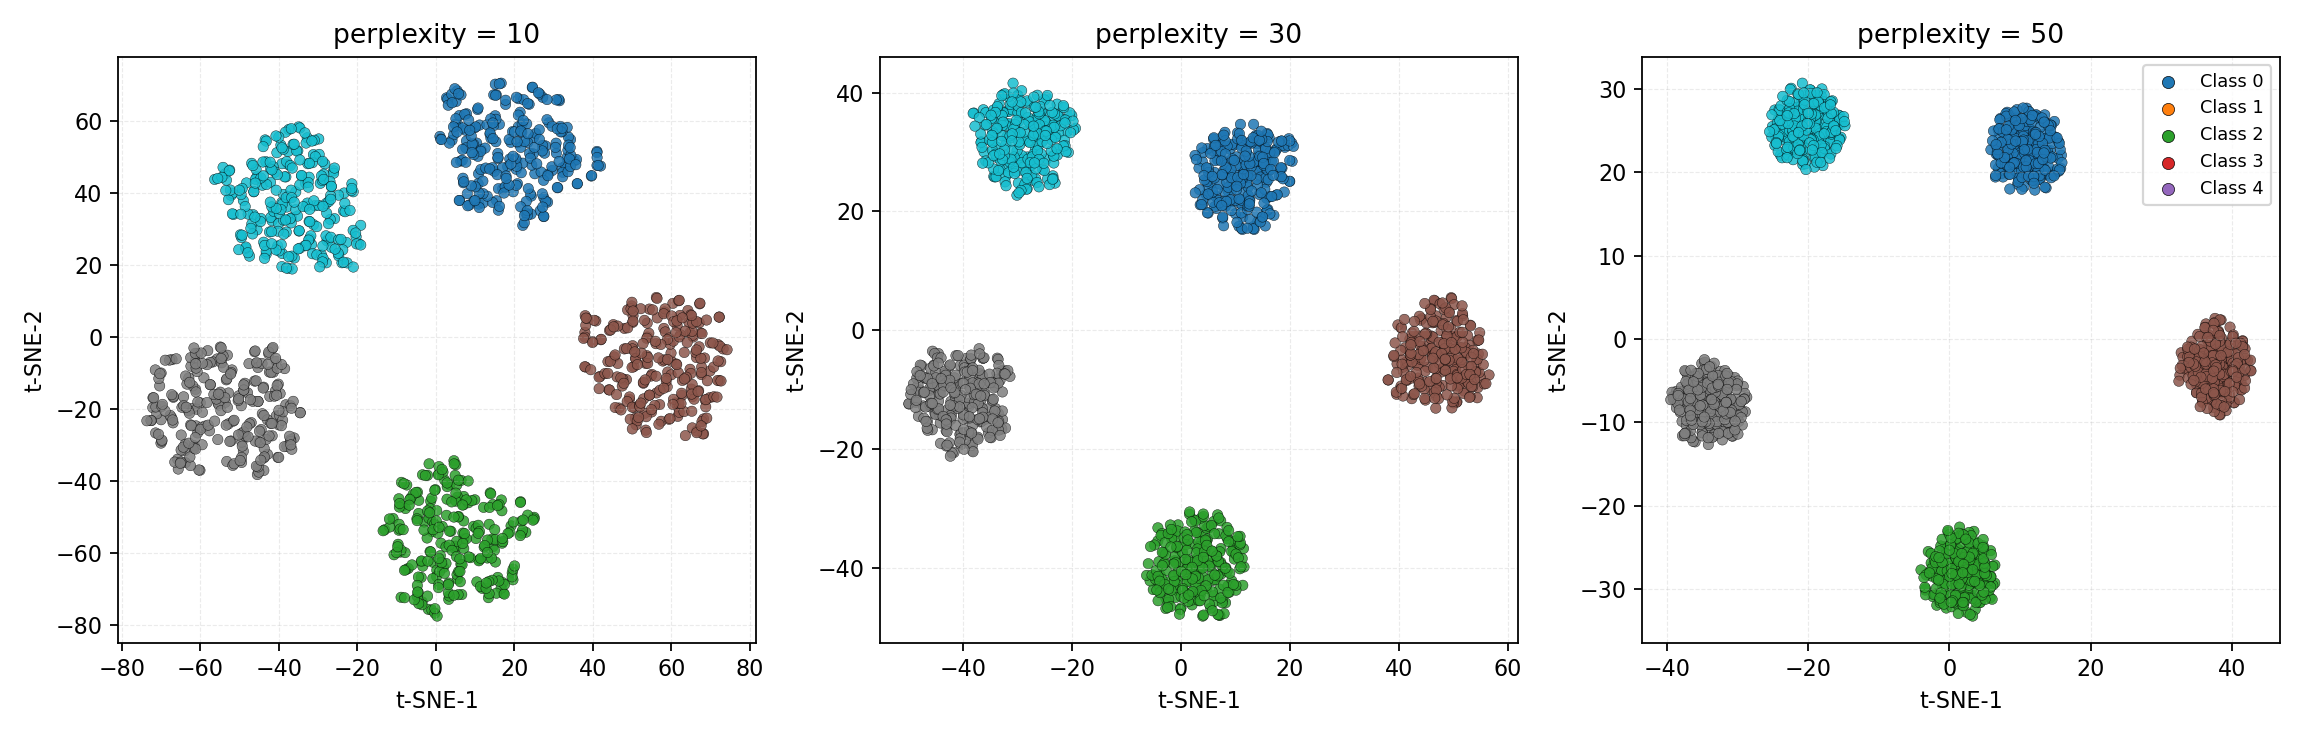
\includegraphics[width=0.82\linewidth]{tsne_embeddings.png}
  \caption{不同困惑度下的 t-SNE 嵌入,可按类别着色}
  \label{fig:tsne_embeddings_cn}
\end{figure}

\begin{figure}[H]
  \centering
  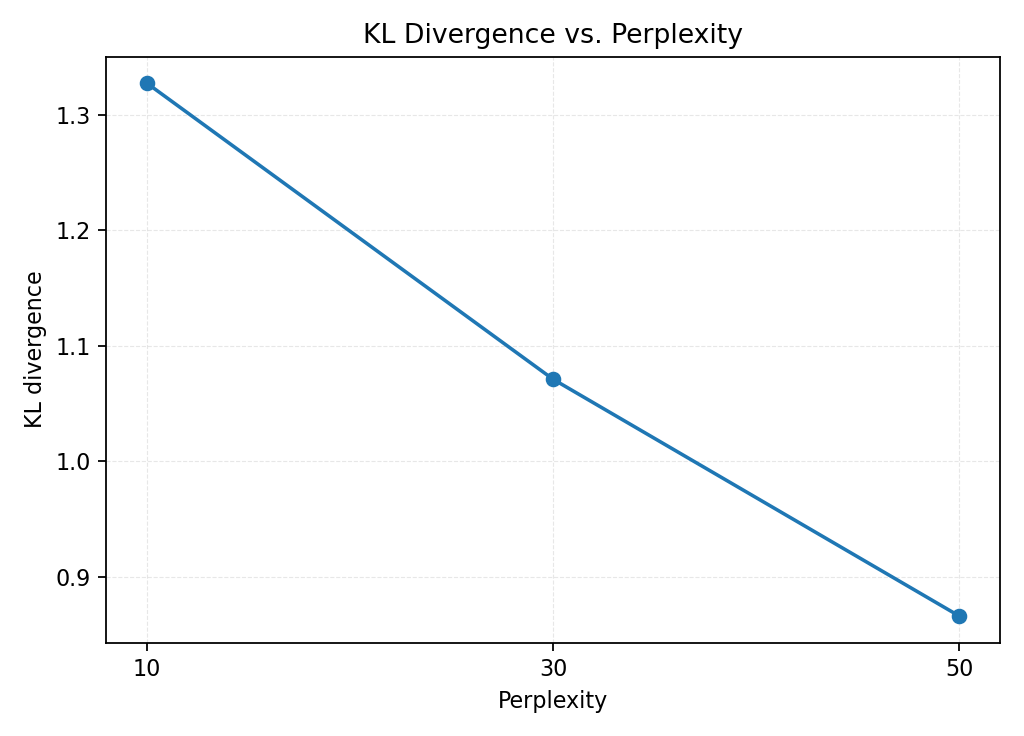
\includegraphics[width=0.8\linewidth]{tsne_perplexity_curve.png}
  \caption{KL 散度随困惑度变化的曲线,用于判断稳定区间}
  \label{fig:tsne_perplexity_curve_cn}
\end{figure}

\FloatBarrier
\section{总结}
t-SNE 通过邻域概率匹配捕获局部结构,减少拥挤效应,实现高维数据的直观可视化。合理调节困惑度、学习率与迭代次数能获得稳定的映射图,辅助探索分析。示例展示了如何比较不同困惑度的嵌入并借助 KL 散度诊断稳定性。

\end{document}
